\documentclass[preview]{standalone}
\usepackage{tkz-graph}
\begin{document}

% \begin{figure}[ht]
% \center
%  \begin{tikzpicture}
%    \draw[->] (0,0) -- (9,0);
%    \draw[->] (0,0) -- (0,5);
%    \draw(-0.2,-0.2) node {$0$};   
%    \draw(8.5,-0.2) node {$x_1$};   
%    \draw(-0.2,4.5) node {$x_2$};      
%    \fill [blue!15] (0,0) rectangle +(8.,4.);   
%    \fill [green!15] (2,2) circle (1);
%    \draw[color=black!50,line width=1pt] (2,2) circle (1);
%    \draw(6.5,2) node {$\Omega_2$};
%    \draw(2,2) node {$\Omega_1$};
%    \draw(3.2,2) node {$\gamma$};
%    \draw[color=red,line width=1pt] (0,0) -- (0,4);
%    \draw[color=blue,line width=1pt] (0,4) -- (8,4) -- (8,0) -- (0,0);
%    \draw(-0.2,2) node {$\Gamma_1$};
%    \draw(8.3,2) node {$\Gamma_2$};
%  \end{tikzpicture}
% \end{figure}

\begin{figure}[ht]
\center
 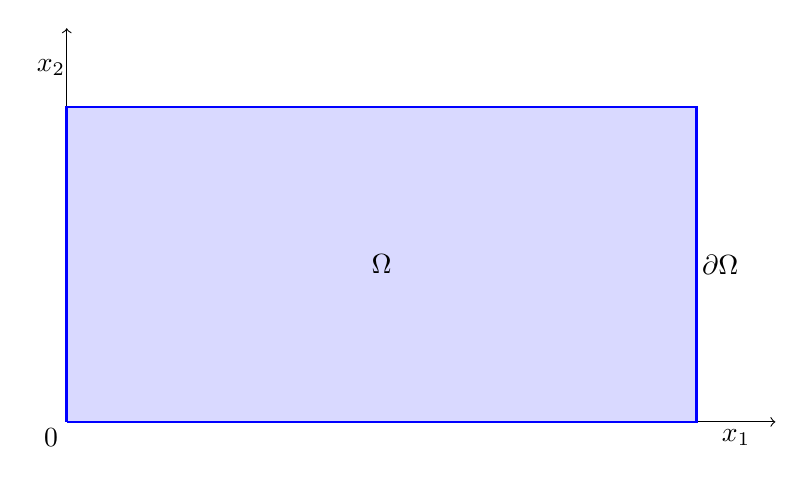
\begin{tikzpicture}
   \draw[->] (0,0) -- (9,0);
   \draw[->] (0,0) -- (0,5);
   \draw(-0.2,-0.2) node {$0$};   
   \draw(8.5,-0.2) node {$x_1$};   
   \draw(-0.2,4.5) node {$x_2$};      
   \fill [blue!15] (0,0) rectangle +(8.,4.);   
   \draw(4,2) node {$\Omega$};
   \draw[color=blue,line width=1pt] (0,0) -- (0,4) -- (8,4) -- (8,0) -- (0,0);
   \draw(8.3,2) node {$\partial\Omega$};
 \end{tikzpicture}
\end{figure}

\end{document}



После: convert pdf to png
https://convertio.co/pdf-png/



 






